\definecolor{green}{RGB}{0,190,0}
\definecolor{red}{RGB}{190,0,0}
\definecolor{gray}{RGB}{35,10,10}

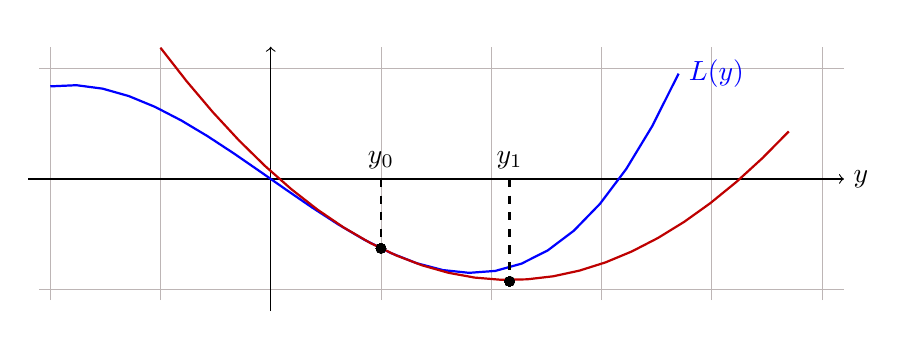
\begin{tikzpicture}[scale = 1.4,domain=-2:3.7]
	\def \point {1};
	
	%Gitter zeichnen
	\draw[very thin,color=gray!30] (-2.1,-1.1) grid (5.2,1.2);
	%Achsen zeichnen
	\draw[->] (-2.2,0) -- (5.2,0) node[right] {$y$};
	\draw[->] (0,-1.2) -- (0,1.2) node[above] {};
	%Funktion zeichnen
	\draw[thick, color=blue] plot (\x, {0.07*(\x)^3 -  0.7*(\x) }) node[right] {$L(y)$};
	\draw[thick, color=red] plot (\x + \point, {(0.5*(0.42*(\point))*(\x)^2 + (0.21*(\point)^2-0.7)*(\x))  +(0.07*(\point)^3 -  0.7*(\point) )} );
%	\draw[thick, color=green] plot (\x , {((0.21*(\point)^2-0.7) + (0.42*(\point))*(\x)) });
%	\draw[thick, mark=x] plot (\point , {(0.07*(\point)^3 -  0.7*(\point) )}) ;
	\draw[thick, dashed] (\point ,0) node[above] {$y_0$} -- (\point,{(0.07*(\point)^3 -  0.7*(\point) )}) ;
%	\draw[thick, decorate, decoration={brace,amplitude=6pt}] (0,0) -- ({- (0.21*(\point)^2-0.7)/(0.42*(\point))},0) node[midway, above,yshift=3pt,]{$s_k$};
	\draw[thick, mark=*, mark size=1pt] plot (\point , {(0.07*(\point)^3 -  0.7*(\point) )}) ;
	\draw[thick] plot ({\point - (0.21*(\point)^2-0.7)/(0.42*(\point))} , 0) node[above] {$y_{1}$};
	\draw[thick, dashed] ({\point - (0.21*(\point)^2-0.7)/(0.42*(\point))} , 0) --++ (0,-0.93);
	\draw[thick, mark=*, mark size=1pt] plot ({\point - (0.21*(\point)^2-0.7)/(0.42*(\point))},-0.93);
	
	%\draw[thick, color=black] plot (\x, {0.21*(\x)^2 -  0.7 });
	\end{tikzpicture}
	
%	\begin{tikzpicture}[domain=-2:4]
%	\def \point {1};
%	
%	%Gitter zeichnen
%	\draw[very thin,color=gray!30] (-2.1,-1.1) grid (5.2,2.2);
%	%Achsen zeichnen
%	\draw[->] (-2.2,0) -- (5.2,0) node[right] {$y$};
%	\draw[->] (0,-1.2) -- (0,2.2) node[above] {$L(y)$};
%	%Funktion zeichnen
%	\draw[thick, color=blue] plot (\x, {0.07*(\x)^3 -  0.7*(\x) });
%	\draw[thick, color=red] plot (\x + \point, {(0.5*(0.42*(\point))*(\x)^2 + (0.21*(\point)^2-0.7)*(\x))  +(0.07*(\point)^3 -  0.7*(\point) )} );
%	\draw[thick, color=green] plot (\x , {((0.21*(\point)^2-0.7) + (0.42*(\point))*(\x)) });
%	\draw[thick, mark=x] plot (\point , {(0.07*(\point)^3 -  0.7*(\point) )}) ;
%	\draw[thick, decorate, decoration={brace,amplitude=6pt}] (0,0) -- ({- (0.21*(\point)^2-0.7)/(0.42*(\point))},0) node[midway, above,yshift=3pt,]{$s_k$};
%	
%%	\draw[thick, mark=x] plot ({\point - (0.21*(\point)^2-0.7)/(0.42*(\point))} , 0) node[below] {$y_{k+1}$};
%	
%	%\draw[thick, color=black] plot (\x, {0.21*(\x)^2 -  0.7 });
%	\end{tikzpicture}